%%%%%%%%%%%%%%%%%%%%%%%%%%%%%%%%%%%%%%%%%%%%%%%%%%%%%%%%%%%%%%%%%%%%%%%
%      Paper A
%%%%%%%%%%%%%%%%%%%%%%%%%%%%%%%%%%%%%%%%%%%%%%%%%%%%%%%%%%%%%%%%%%%%%%%
\section{Paper A}
\section*{Finite Element solution of the fiber/matrix interface crack problem: convergence properties and mode mixity of the Virtual Crack Closure Technique}

The analysis of bi-material interface cracks, such as the fiber/matrix interface crack or debond, in the context of Linear Elastic Fracture Mechanics hides some peculiar complexities due to the nature of the solution at the crack tip. The solution to the fiber/matrix interface crack problem can be classified into two different regimes~\cite{Paris1996,Varna1997a}: the \emph{open crack} and \emph{closed crack} solution. The distinction between the two lies in the existence of a region of contact between crack faces (contact zone) at the crack tip: if it exists, we talk about a \emph{closed crack} solution, otherwise of an \emph{open crack} solution.\\
The \emph{open crack} solution to the straight bi-material interface crack problem was first proposed by Williams~\cite{Williams1959}, who found the existence of an oscillatory singularity in the stress field at the crack tip of the form

\begin{equation}\label{chap3:paperA:eq:singularitywilliams}
r^{-\frac{1}{2}}\sin\left(\varepsilon\log r\right)\quad\text{with}\quad\varepsilon=\frac{1}{2\pi}\log\left(\frac{1-\beta}{1+\beta}\right),
\end{equation}

in both Mode I and Mode II. In Eq.~\ref{chap3:paperA:eq:singularitywilliams}, $\beta$ is one of the two parameters introduced by Dundurs~\cite{Dundurs1969} to characterize bi-material interfaces:

\begin{equation}\label{chap3:paperA:eq:dundursbeta}
\beta=\frac{\mu_{2}\left(\kappa_{1}-1\right)-\mu_{1}\left(\kappa_{2}-1\right)}{\mu_{2}\left(\kappa_{1}+1\right)+\mu_{1}\left(\kappa_{2}+1\right)}
\end{equation}

where $\kappa=3-4\nu$ in plane strain and $\kappa=\frac{3-4\nu}{1+\nu}$ in plane stress, $\mu$ is the shear modulus, $\nu$ Poisson's coefficient, and indexes $1,2$ refer to the two bulk materials joined at the interface. Due to the nature of singular solution at the crack tip in the \emph{open crack} case, the definition of Stress Intensity Factor (SIF) $\lim_{r\rightarrow 0}\sqrt{2\pi r}\sigma$ diverges and is not anymore valid~\cite{Comninou1990}. The mismatch in the value of the elastic properties at the bi-material interface makes the configuration a mixed-mode one, but the Mode mixity problem at the crack tip is ill-posed. For the same reason, Mode I and Mode II Energy Release Rate do not converge. A way to circumvent the problem is to evaluate the ERR over a finite instead of an infinitesimal crack increment, which leads naturally to the application of the Virtual Crack Closure Technique (VCCT)~\cite{Rybicki1977,Krueger2004}.\\
The introduction of a finite crack increment makes the ERR sensitive to the mesh. Several authors have investigated the mesh sensitivity of the VCCT used in conjunction with the Finite Element Method (FEM) in the context of the straight bi-material interface crack~\cite{Krueger2013,Sun1987,Sun1989,Manoharan1990,Raju1988,Agrawal2006,Wang2013} and found that: the total Energy Release Rate $G_{TOT}$ does not depend on the mesh size; for a crack under mixed-mode behavior (\emph{open crack} case), Mode I and Mode II depend on the size of the mesh at the crack tip and do not show convergence. The purpose of this first paper is to analyze the mesh dependency of Energy Release Rate in the case of the fiber/matrix interface crack.

\begin{figure}[!h]
\centering
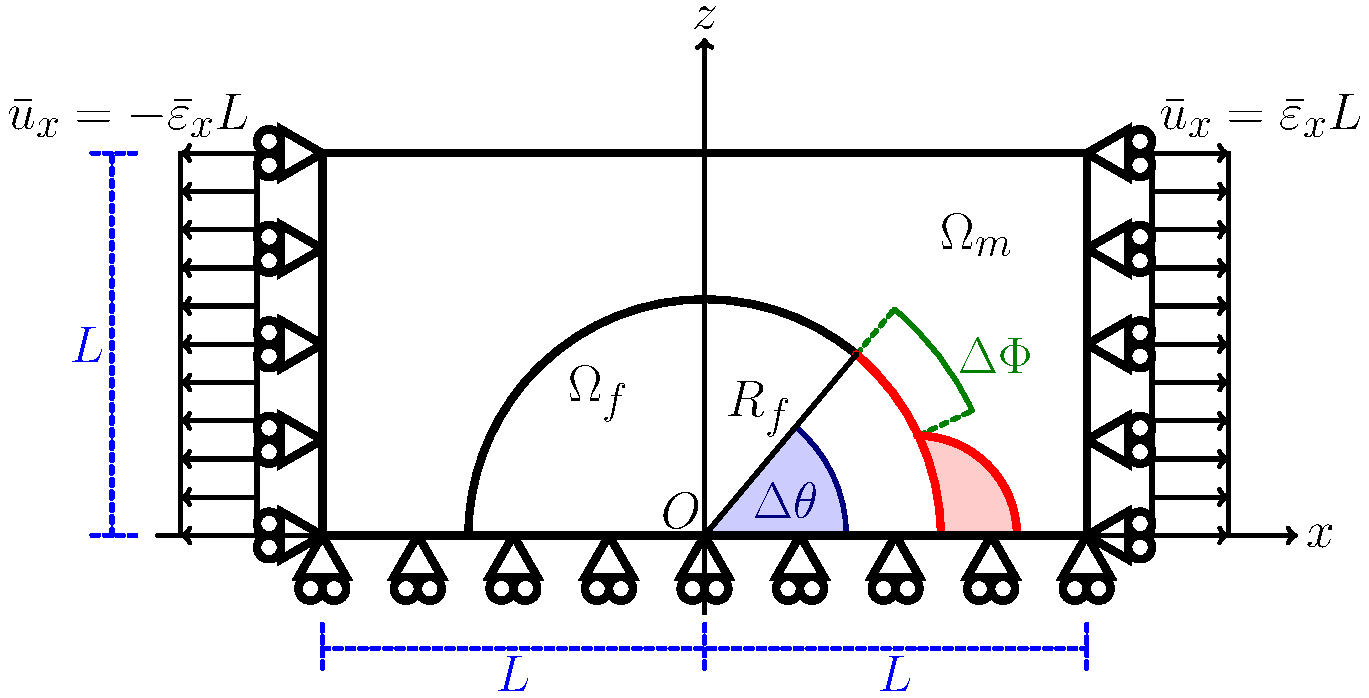
\includegraphics[width=\textwidth]{paperA/RUC.pdf}
\caption{Schematic of the model with its main parameters.}\label{chap3:paperA:fig:modelschem}
\end{figure}

The 1-step VCCT in the force-displacement formulation~\cite{Krueger2004} is considered and applied to the evaluation of the ERR of a debond located on a single fiber placed in a square matrix cell, as shown in Figure~\ref{chap3:paperA:fig:modelschem}. The cell has a size of $2L\times2L$, where

\begin{equation}\label{chap3:paperA:eq:LVf}
L=\frac{R_{f}}{2}\sqrt{\frac{\pi}{V_{f}}},
\end{equation}

$V_{f}$ is the fiber volume fraction and $R_{f}$ is the fiber radius, assumed to be equal to $1\ \mu m$. The occurrence of a contact zone after a critical size of the debond is considered and a contact pair interaction is established between crack faces. The interaction is considered frictionless. As the model is symmetric with respect to the $x$-axis (see Figure~\ref{chap3:paperA:fig:modelschem}), only half of it is explicitly modeled and symmetry conditions are applied to the lower boundary. A constant $x$-strain of $1\%$ is applied to the right and left boundary. Glass fiber and epoxy are considered and their properties are reported in Table~\ref{chap3:paperA:tab:phaseprop}.

\begin{table}[!htbp]
 \centering
 \caption{Summary of the mechanical properties of fiber and matrix. $E$ stands for Young's modulus, $\mu$ for shear modulus and $\nu$ for Poisson's ratio.}
 \begin{tabular}{cccc}
\textbf{Material} & \textbf{$E\left[GPa\right]$}\ & \textbf{$\mu\left[GPa\right]$} & \textbf{$\nu\left[-\right]$} \\
\midrule
Glass fiber    & 70.0  & 29.2   & 0.2  \\
Epoxy    & 3.5    & 1.25   & 0.4
\end{tabular}
\label{chap3:paperA:tab:phaseprop}
\end{table}

The main parameter of the mesh sensitivity study is the angular size $\delta$ of the elements at the crack tip, as shown in Figure~\ref{chap3:paperA:fig:vcctmesh}.

\begin{figure}[!h]
\centering
    \begin{subfigure}[b]{0.8\textwidth}
        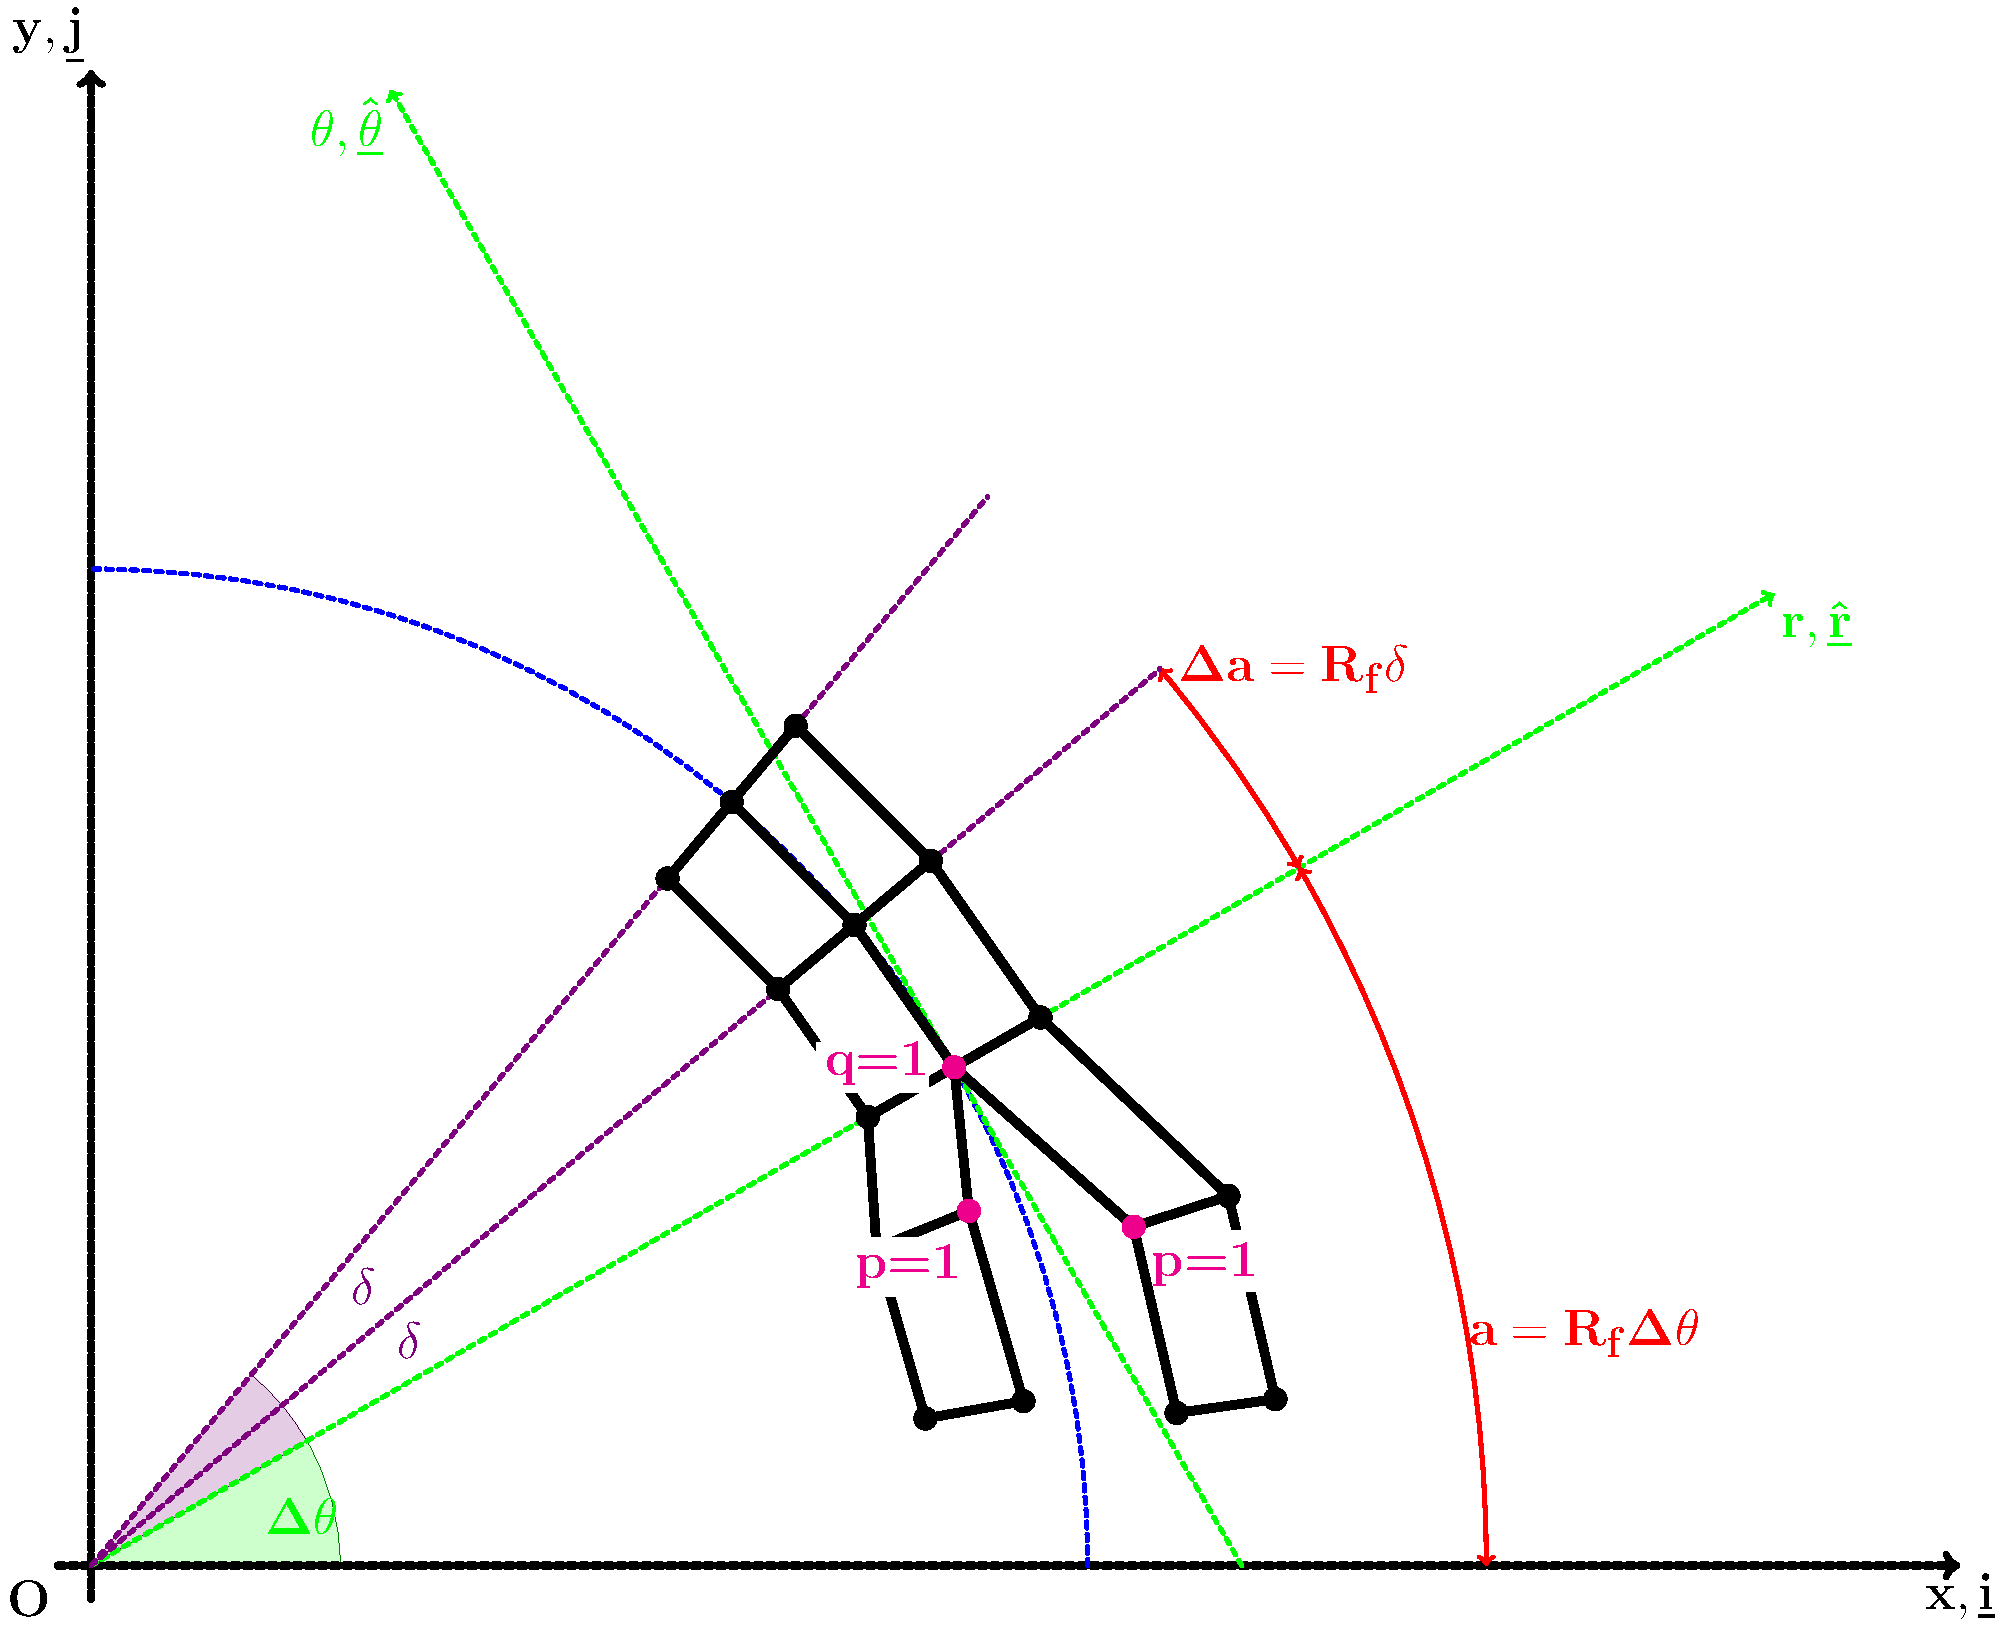
\includegraphics[width=\textwidth]{paperA/VCCT-linear.pdf}
       \caption{\added{Elements with $1^{st}$ order shape functions: $m=1$ and $p,q=1$.}}
    \end{subfigure}

    \begin{subfigure}[b]{0.8\textwidth}
        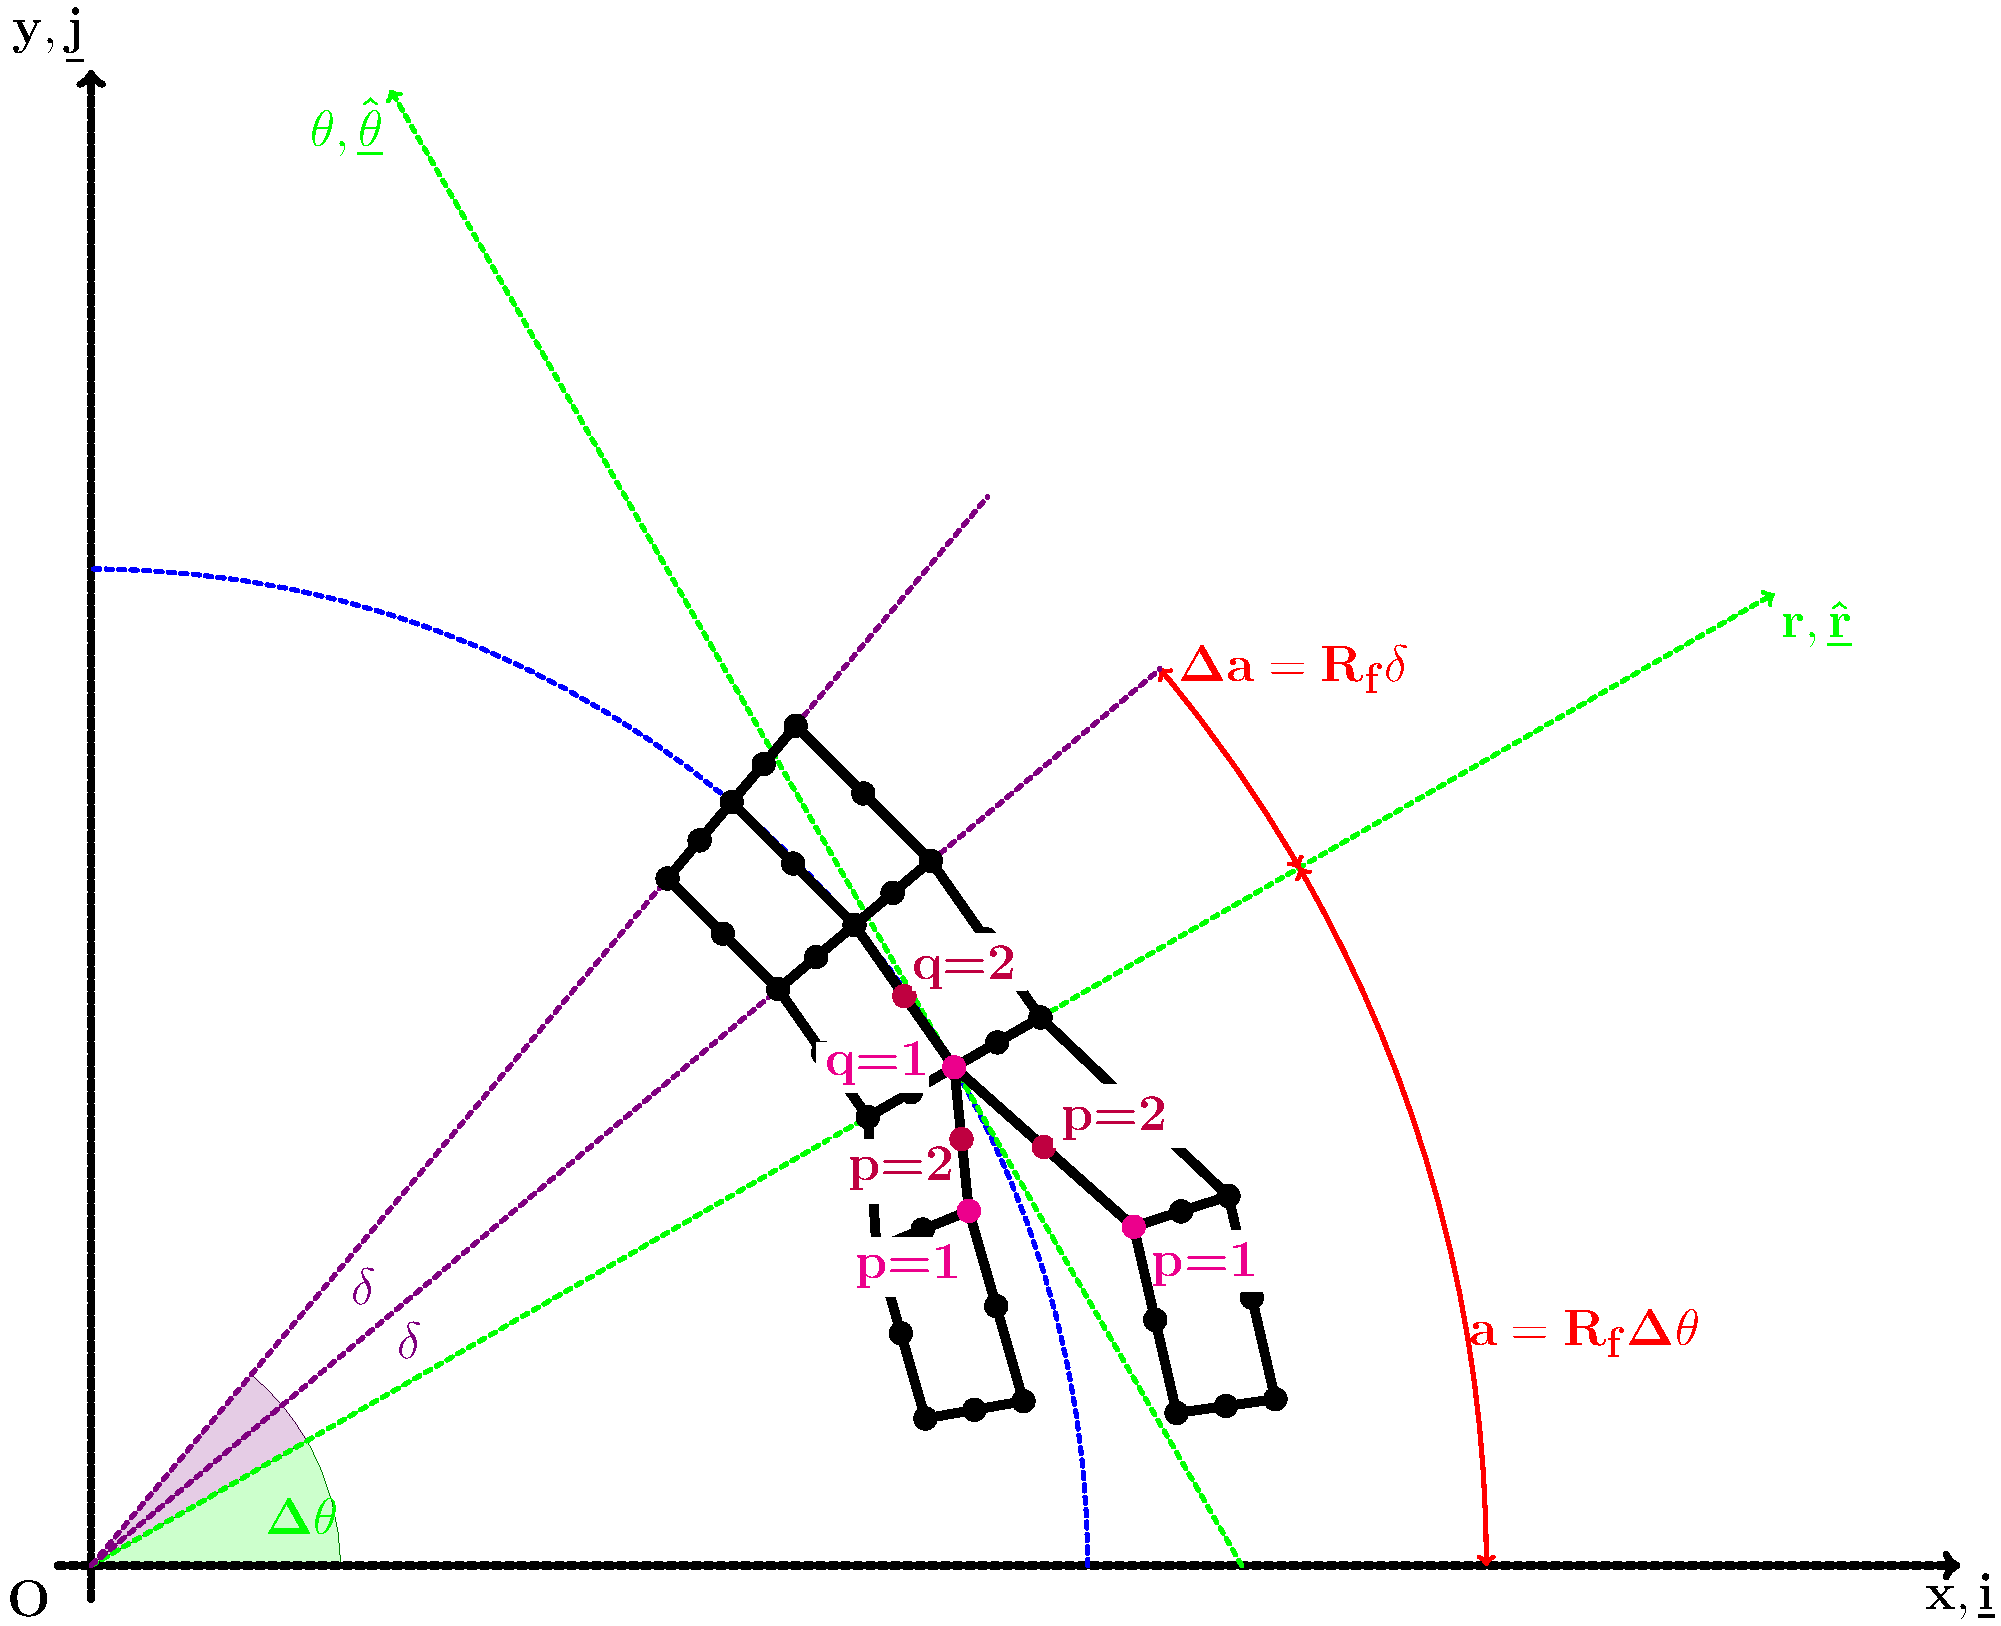
\includegraphics[width=\textwidth]{paperA/VCCT-quadratic.pdf}
       \caption{\added{Elements with $2^{nd}$ order shape functions: $m=2$ and $p,q=1,2$.}}
    \end{subfigure}

\caption{\added{Schematic of the mesh at the fiber/matrix interface crack tip.}}\label{chap3:paperA:fig:vcctmesh}
\end{figure}

\begin{figure}[!h]
\centering
    \begin{subfigure}[b]{0.48\textwidth}
        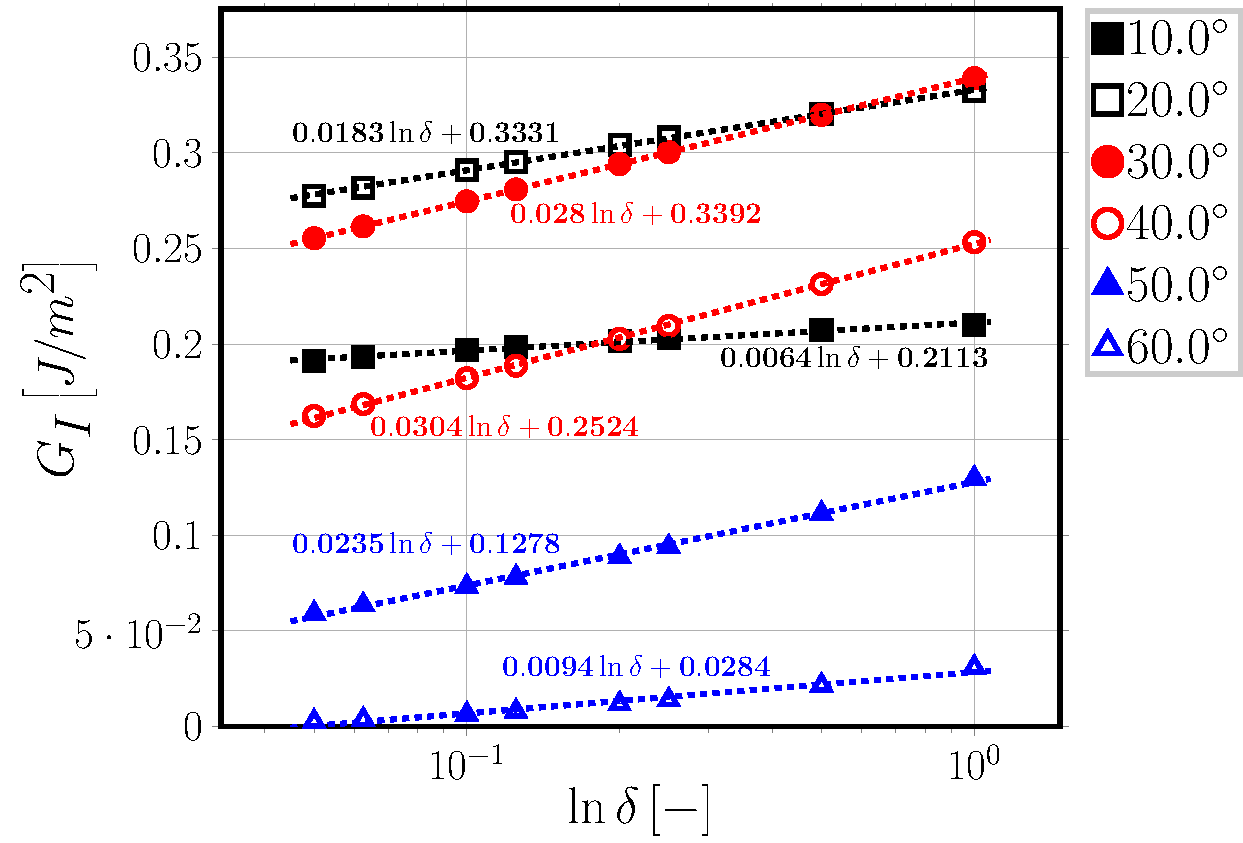
\includegraphics[width=\textwidth]{paperA/Vf0_1-free-1st-semilogvsDelta-GI.pdf}
       \caption{$V_{f}=0.1\%$, $1^{st}$ order elements.}
    \end{subfigure}
    ~
    \begin{subfigure}[b]{0.48\textwidth}
        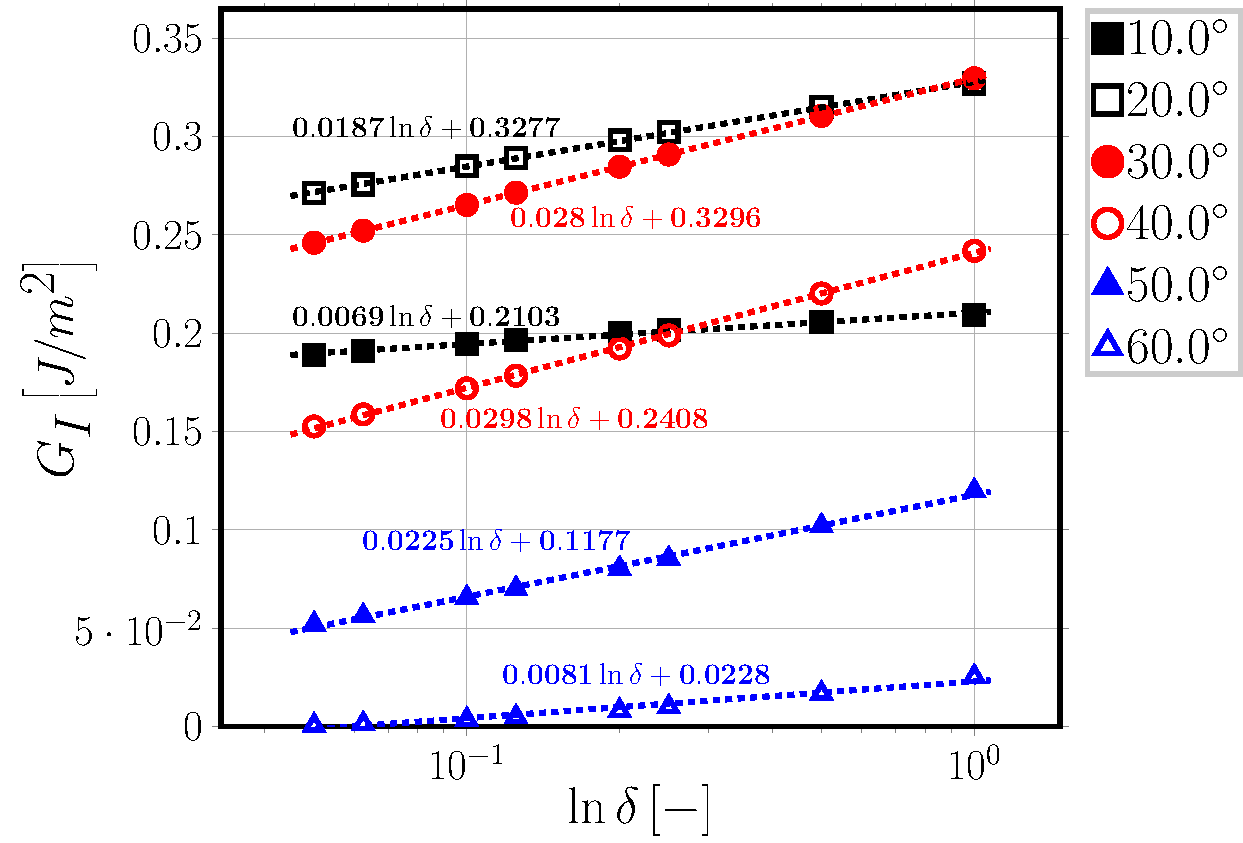
\includegraphics[width=\textwidth]{paperA/Vf0_1-free-2nd-semilogvsDelta-GI.pdf}
       \caption{$V_{f}=0.1\%$, $2^{nd}$ order elements.}
    \end{subfigure}

    \begin{subfigure}[b]{0.48\textwidth}
        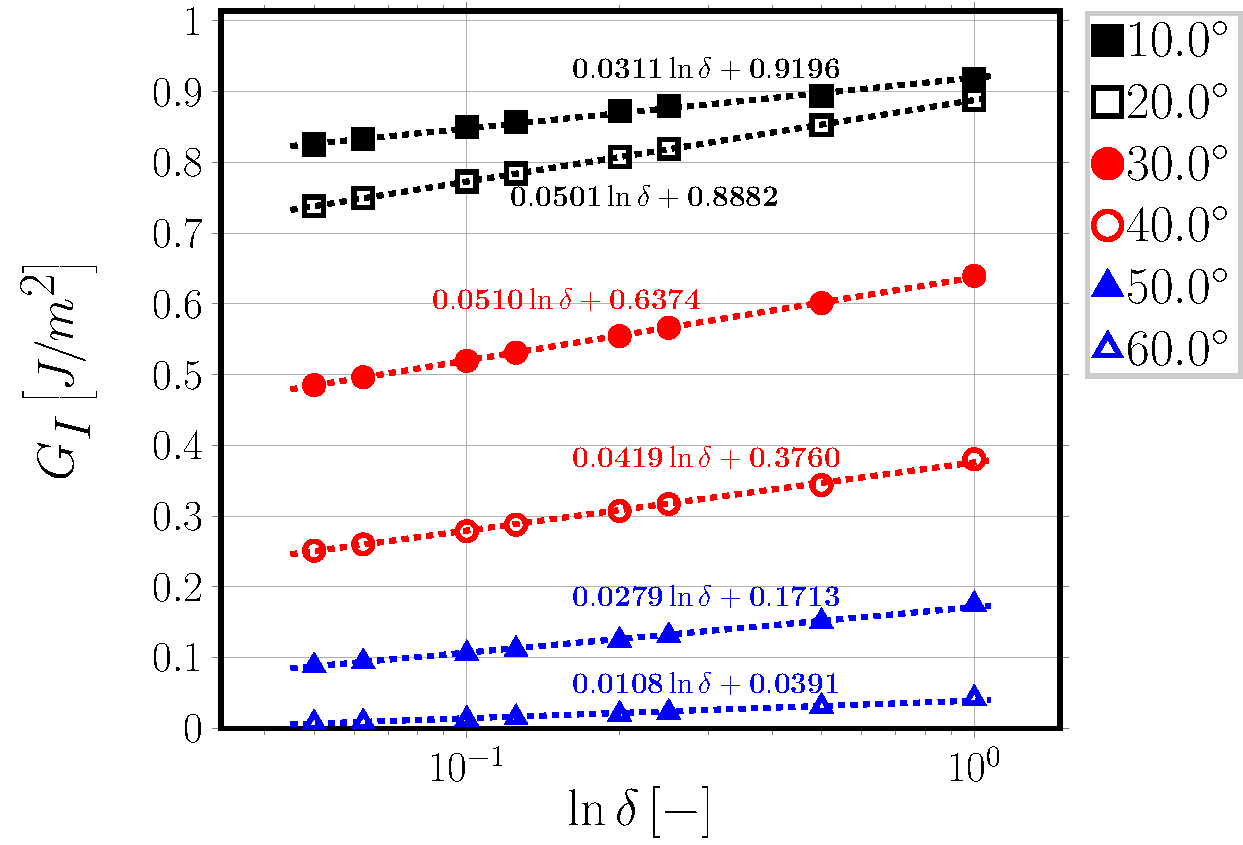
\includegraphics[width=\textwidth]{paperA/Vf40-free-1st-semilogvsDelta-GI.pdf}
       \caption{$V_{f}=40\%$, $1^{st}$ order elements.}
    \end{subfigure}
    ~
    \begin{subfigure}[b]{0.48\textwidth}
        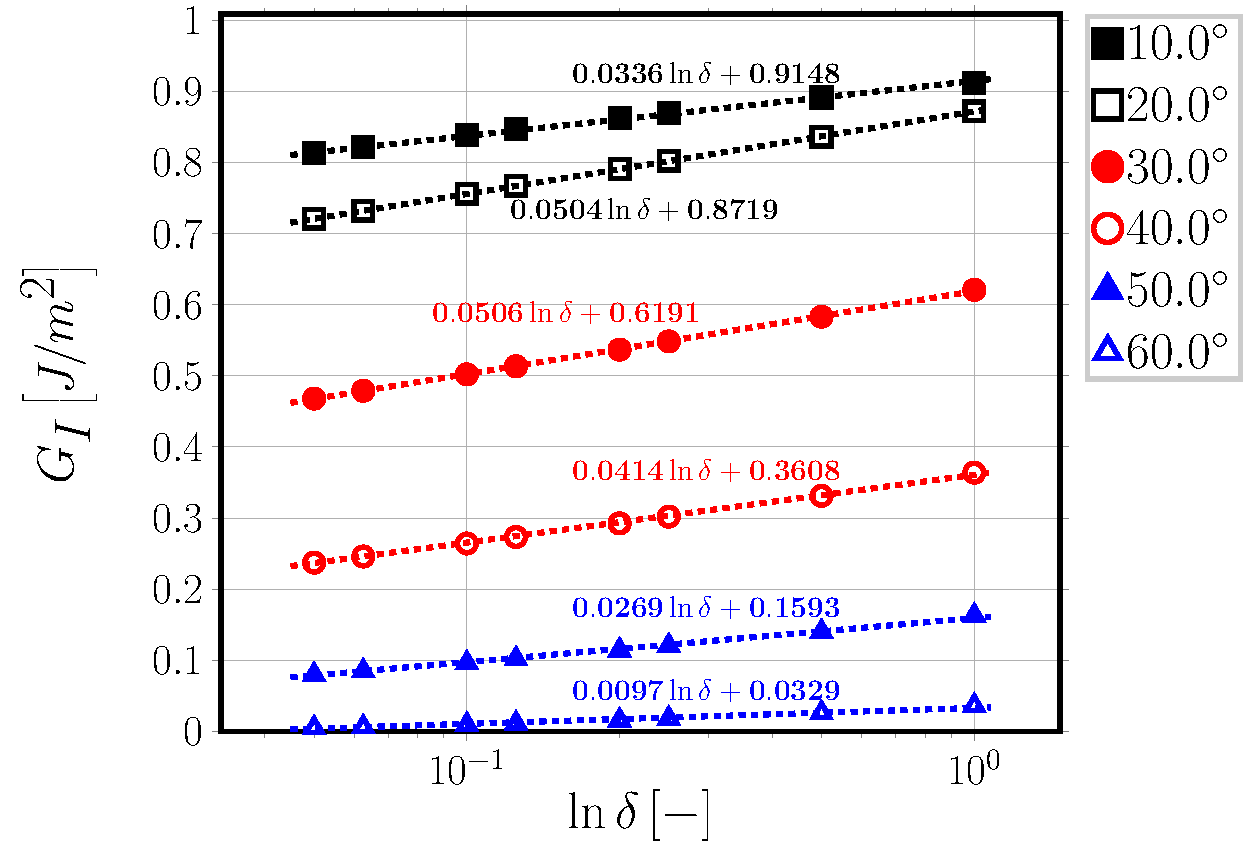
\includegraphics[width=\textwidth]{paperA/Vf40-free-2nd-semilogvsDelta-GI.pdf}
       \caption{$V_{f}=40\%$, $2^{nd}$ order elements.}
    \end{subfigure}

\caption{Logarithmic dependence on $\delta$ of Mode I ERR: interpolation of numerical results.}\label{chap3:paperA:fig:gIinterp}
\end{figure}

\begin{figure}[!h]
\centering
    \begin{subfigure}[b]{0.48\textwidth}
        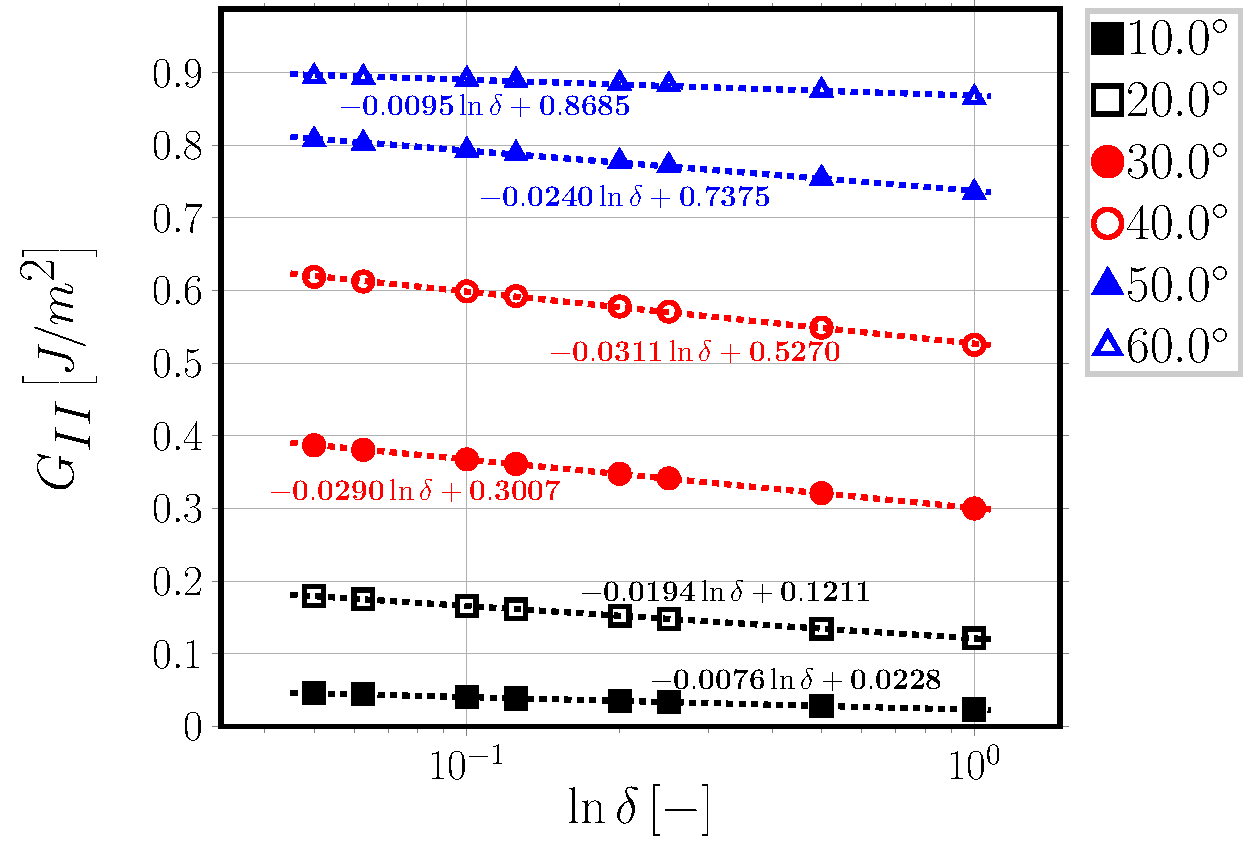
\includegraphics[width=\textwidth]{paperA/Vf0_1-free-1st-semilogvsDelta-GII.pdf}
       \caption{$V_{f}=0.1\%$, $1^{st}$ order elements.}
    \end{subfigure}
    ~
    \begin{subfigure}[b]{0.48\textwidth}
        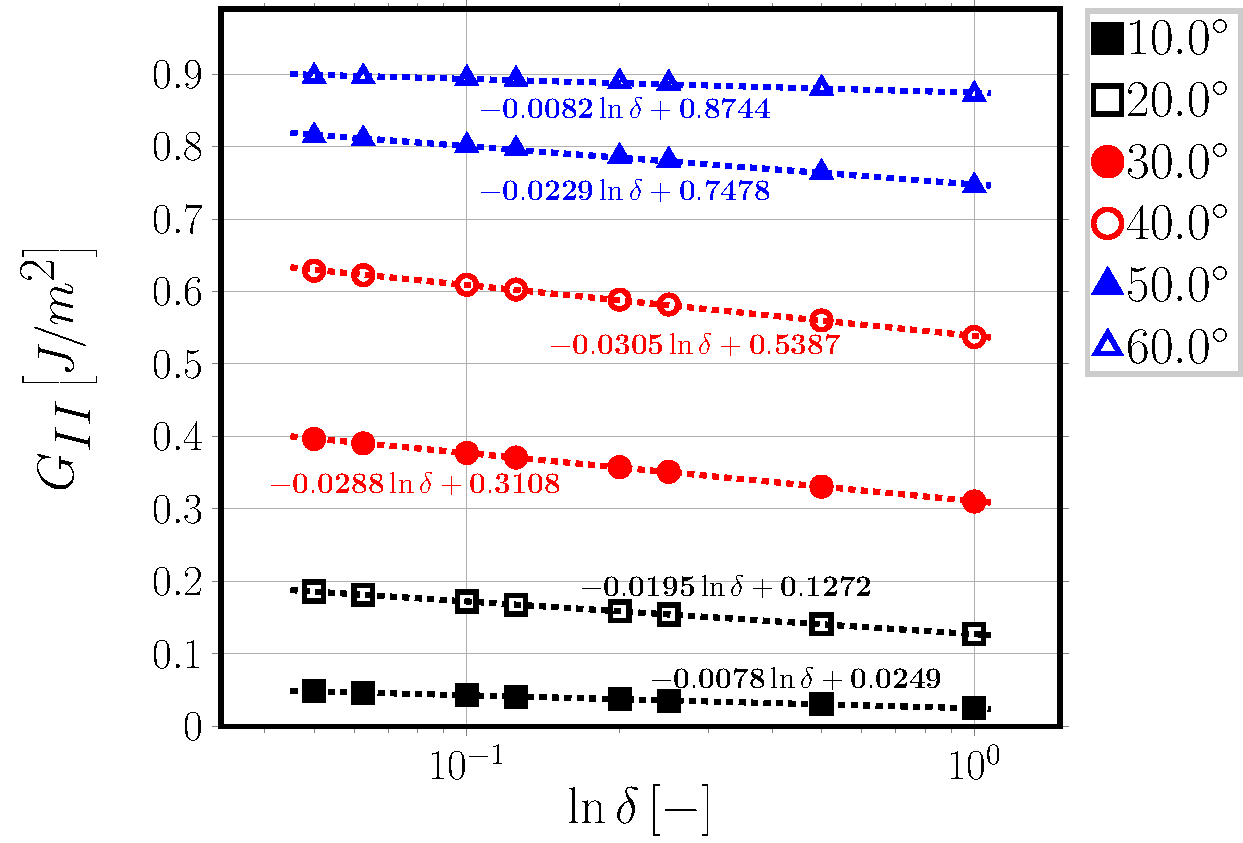
\includegraphics[width=\textwidth]{paperA/Vf0_1-free-2nd-semilogvsDelta-GII.pdf}
       \caption{$V_{f}=0.1\%$, $2^{nd}$ order elements.}
    \end{subfigure}

    \begin{subfigure}[b]{0.48\textwidth}
        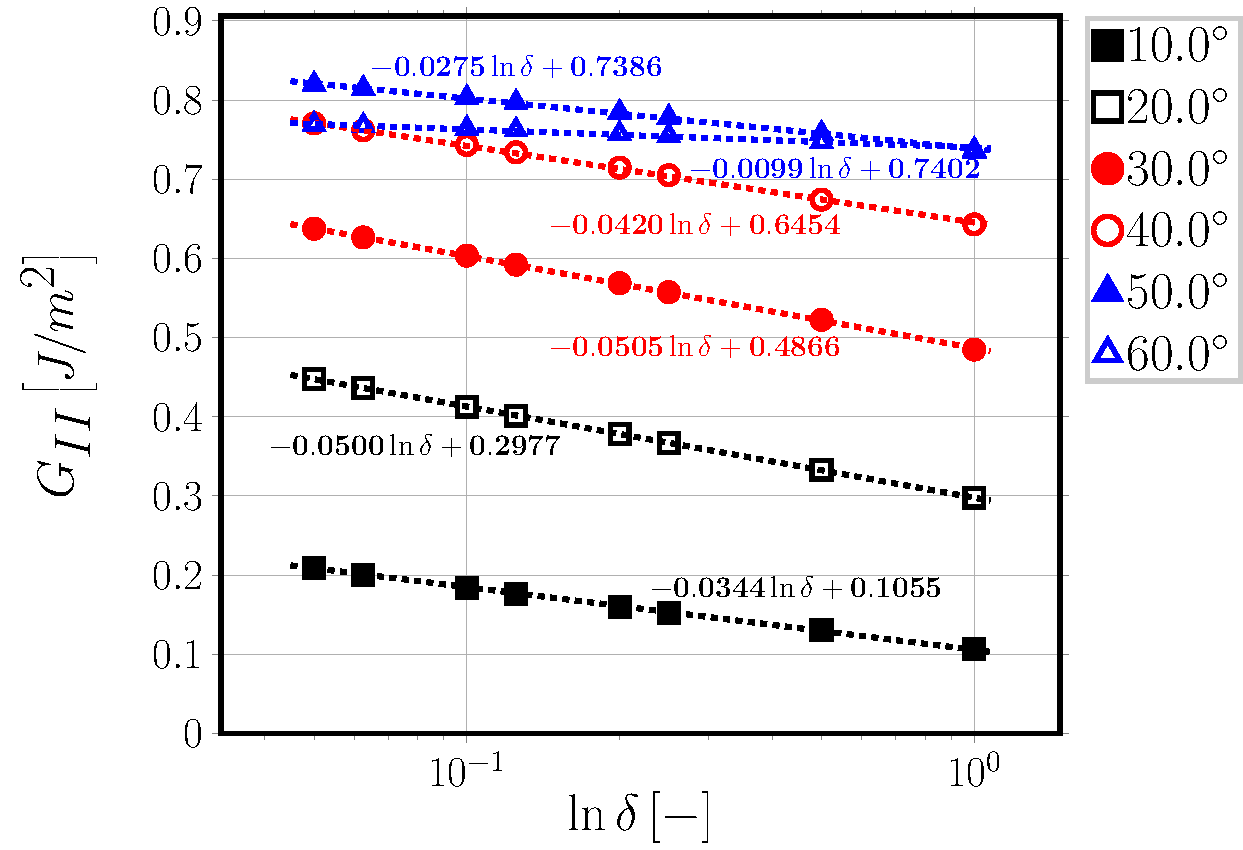
\includegraphics[width=\textwidth]{paperA/Vf40-free-1st-semilogvsDelta-GII.pdf}
       \caption{$V_{f}=40\%$, $1^{st}$ order elements.}
    \end{subfigure}
    ~
    \begin{subfigure}[b]{0.48\textwidth}
        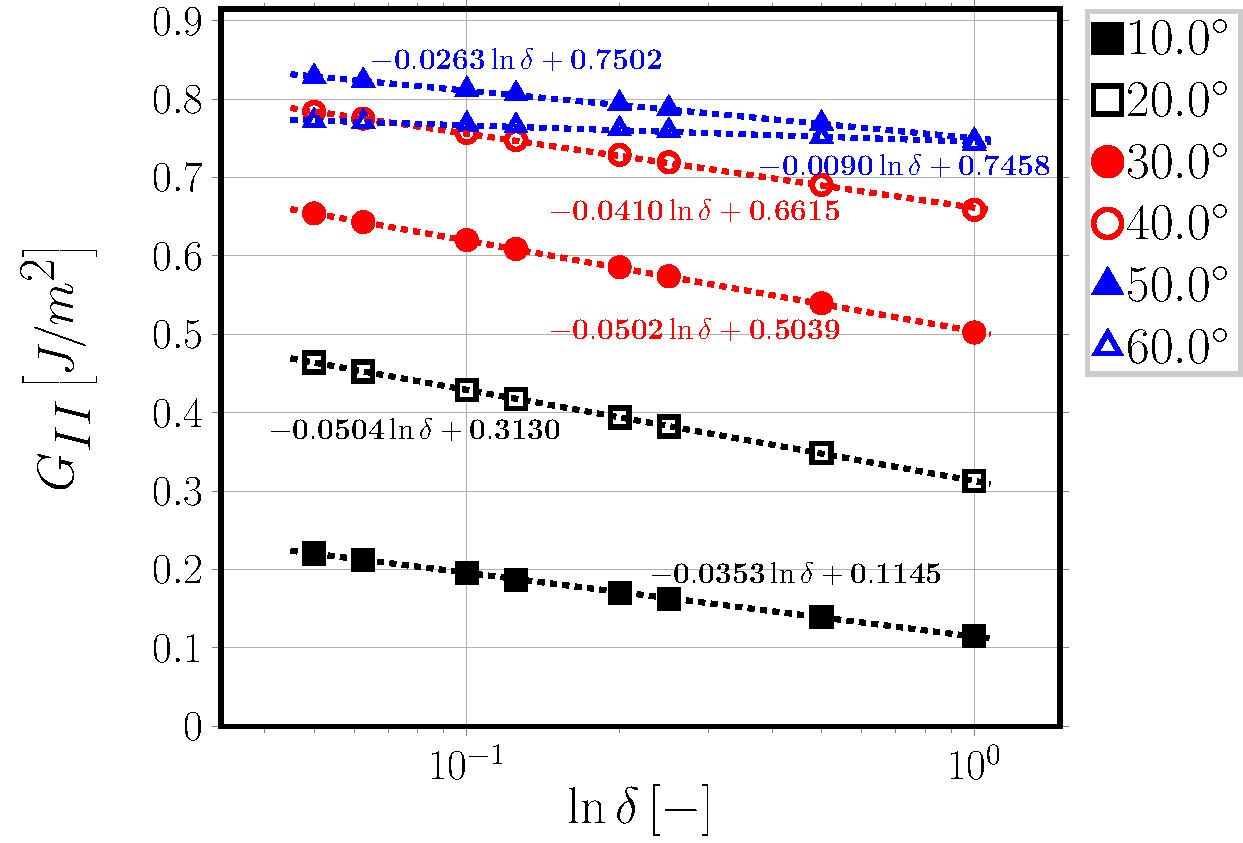
\includegraphics[width=\textwidth]{paperA/Vf40-free-2nd-semilogvsDelta-GII.pdf}
       \caption{$V_{f}=40\%$, $2^{nd}$ order elements.}
    \end{subfigure}

\caption{Logarithmic dependence on $\delta$ of Mode II ERR: interpolation of numerical results.}\label{chap3:paperA:fig:gIIinterp}
\end{figure}

It is found in Paper A that

\begin{itemize}
\item the total ERR is invariant to rotations of the reference frame (and more in general to linear transformations), which implies that rotation of crack tip forces and displacement is actually not required in the use of the VCCT for the calculation of $G_{TOT}$;
\item the total ERR does not depend on the size $\delta$ of the elements at the crack tip, at least for reasonably small elements ($\delta\leq1.0^{\circ}$) ;
\item as a consequence, Mode II ERR for the \emph{closed} interface crack does not depend on $\delta$, as $G_{II}=G_{TOT}$ after the onset of the contact zone;
\item for the \emph{open} interface crack, Mode I and Mode II ERR depend on the element size $\delta$ through a logarithmic law of the type $A\left(\Delta\theta\right)\ln\delta+B\left(\Delta\theta\right)$, as shown in Figure~\ref{chap3:paperA:fig:gIinterp} and Figure~\ref{chap3:paperA:fig:gIIinterp};
\item the sign of the logarithm is always positive for $G_{I}$ (see Figure~\ref{chap3:paperA:fig:gIinterp}), i.e. it decreases when $\delta$ decreases, and negative for $G_{II}$ (see Figure~\ref{chap3:paperA:fig:gIIinterp}), i.e. it increases when $\delta$ decreases.
\end{itemize}


%%%%%%%%%%%%%%%%%%%%%%%%%%%%%%%%%%%%%%%%%%%%%%%%%%%%%%%%%%%%%%%%%%%%%%%
%      Paper B
%%%%%%%%%%%%%%%%%%%%%%%%%%%%%%%%%%%%%%%%%%%%%%%%%%%%%%%%%%%%%%%%%%%%%%%
\section{Paper B}
\section*{Energy release rate of the fiber/matrix interface crack in UD composites under transverse loading: effect of the fiber volume fraction and of the distance to the free surface and to non-adjacent debonds}

%%%%%%%%%%%%%%%%%%%%%%%%%%%%%%%%%%%%%%%%%%%%%%%%%%%%%%%%%%%%%%%%%%%%%%%
%      Paper C
%%%%%%%%%%%%%%%%%%%%%%%%%%%%%%%%%%%%%%%%%%%%%%%%%%%%%%%%%%%%%%%%%%%%%%%
\section{Paper C}
\section*{Effect of the proximity to the $\mathbf{0^{\circ}/90^{\circ}}$ interface on Energy Release Rate of fiber/matrix interface crack growth in the  $\mathbf{90^{\circ}}$-ply of a cross-ply laminate under tensile loading}

%%%%%%%%%%%%%%%%%%%%%%%%%%%%%%%%%%%%%%%%%%%%%%%%%%%%%%%%%%%%%%%%%%%%%%%
%      Paper D
%%%%%%%%%%%%%%%%%%%%%%%%%%%%%%%%%%%%%%%%%%%%%%%%%%%%%%%%%%%%%%%%%%%%%%%
\section{Paper D}
\section*{Growth of interface cracks on consecutive fibers: on the same or on the opposite sides?}

%%%%%%%%%%%%%%%%%%%%%%%%%%%%%%%%%%%%%%%%%%%%%%%%%%%%%%%%%%%%%%%%%%%%%%%
%      Paper E
%%%%%%%%%%%%%%%%%%%%%%%%%%%%%%%%%%%%%%%%%%%%%%%%%%%%%%%%%%%%%%%%%%%%%%%
\section{Paper E}
\section*{Estimating the average size of fiber/matrix interface cracks in ud and cross-ply laminates}
